\documentclass[10pt]{standalone}
\usepackage{times}
\usepackage{amsmath,amssymb,xspace,xcolor,tikz}
\usetikzlibrary{arrows.meta,positioning,shapes.geometric,calc,fit,backgrounds,decorations.pathmorphing}

\newcommand{\todo}[1]{{\color{red}#1}}
\newcommand{\TODO}[1]{\textbf{\color{red}[TODO: #1]}}
\newcommand{\method}{CxWM\xspace}
\newcommand{\vjepa}{V-JEPA~2.1\xspace}
\newcommand{\flywire}{FlyWire\xspace}
\providecommand{\etal}{\emph{et al}.\xspace}
\providecommand{\ie}{\emph{i.e}.\xspace}
\providecommand{\eg}{\emph{e.g}.\xspace}
\newcommand{\degree}{$^\circ$}
\let\mathpm\pm
\renewcommand{\pm}{\ensuremath{\mathpm}}

% diagram colours (populations match the released 3-D viewer)
\definecolor{cVIS}{RGB}{66,133,244}
\definecolor{cCX}{RGB}{244,160,0}
\definecolor{cMB}{RGB}{52,168,83}
\definecolor{cOUT}{RGB}{219,68,155}
\definecolor{cTeach}{RGB}{90,90,90}
\tikzset{
  box/.style={draw,rounded corners=2pt,minimum height=1.6em,inner sep=4pt,font=\small,align=center},
  pop/.style={box,fill=#1!15,draw=#1!80!black,thick},
  arr/.style={-{Latex[length=2mm]},thick},
  darr/.style={-{Latex[length=2mm]},thick,dashed},
  lbl/.style={font=\scriptsize,align=center},
}
\begin{document}
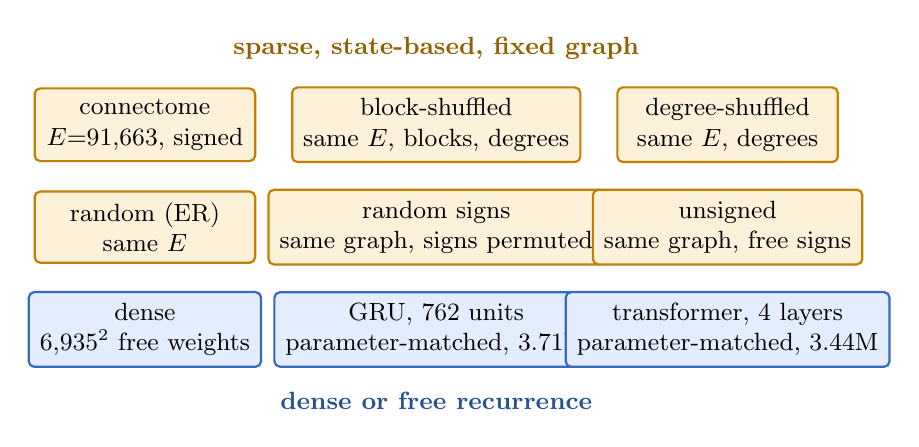
\begin{tikzpicture}[x=3.7cm,y=1.3cm]
    \node[pop=cCX,minimum width=2.8cm] at (0,2) (c) {connectome\\$E{=}91{,}663$, signed};
    \node[pop=cCX,minimum width=2.8cm] at (1,2) (bs) {block-shuffled\\same $E$, blocks, degrees};
    \node[pop=cCX,minimum width=2.8cm] at (2,2) (ds) {degree-shuffled\\same $E$, degrees};
    \node[pop=cCX,minimum width=2.8cm] at (0,1) (er) {random (ER)\\same $E$};
    \node[pop=cCX,minimum width=2.8cm] at (1,1) (rs) {random signs\\same graph, signs permuted};
    \node[pop=cCX,minimum width=2.8cm] at (2,1) (us) {unsigned\\same graph, free signs};
    \node[pop=cVIS,minimum width=2.8cm] at (0,0) (dn) {dense\\$6{,}935^2$ free weights};
    \node[pop=cVIS,minimum width=2.8cm] at (1,0) (gru) {GRU, 762 units\\parameter-matched, 3.71M};
    \node[pop=cVIS,minimum width=2.8cm] at (2,0) (tf) {transformer, 4 layers\\parameter-matched, 3.44M};
    \node[lbl,font=\small\bfseries,cCX!60!black] at (1,2.75) {sparse, state-based, fixed graph};
    \node[lbl,font=\small\bfseries,cVIS!60!black] at (1,-0.7) {dense or free recurrence};
  \end{tikzpicture}
\end{document}
